\documentclass[times, utf8, zavrsni]{fer}
\usepackage{booktabs}
\usepackage[utf8]{inputenc}
\usepackage{graphicx}
\usepackage{amsmath}
\usepackage{algpseudocode}
\usepackage{mathtools}
\pagestyle{empty}
\setlength{\arrayrulewidth}{1mm}
\setlength{\tabcolsep}{18pt}
\renewcommand{\arraystretch}{1.5}
\graphicspath{ {./images/} }

\usepackage{physics}

\thesisnumber{0}
\title{Genetski algoritmi inspirirani kvantnom mehanikom}
\author{Juraj Fulir}

\begin{document}
\maketitle
\section{Originalni zadatak}
Opisati paradigmu kvantnog računanja i primjenu kvantnih računala u postupcima optimizacije. Istražiti mogućnosti oblikovanja stohastičkih optimizacijskih algoritama uz korištenje simulacije rada kvantnog računala. Implementirati nekoliko primjera kvantnih optimizacijskih algoritama koristeći postojeći programski okvir za evolucijsko računanje. Ispitati učinkovitost ostvarenih algoritama i usporediti s postojećim optimizacijskim algoritmima. Radu priložiti izvorne tekstove programa, dobivene rezultate uz potrebna objašnjenja i korištenu literaturu.

\newpage

\zahvala{

Zahvaljujem mentoru, prof.dr.sc. Domagoju Jakoboviću na savjetima, mogućnosti samostalnog odabira teme  završnog rada, kao i obitelji i prijateljima na podršci. Također, velika hvala Karlu Kneževiću, mag.ing.comp., na podršci i potpori teme završnog rada. ??????????
}

\tableofcontents


\chapter{Uvod}
Svijet koji svakodnevno iskušavamo djeluje nam deterministički.
Dugo vremena fizičari su mislili jednako, sve do početka 19. stoljeća kada su u središte pažnje svijeta fizike došli do tada neobjašnjivi fenomeni.  ............
\section{Povijest kvantnih algoritama i procesora}
\subsection{Algoritmi}
\subsection{Računala}
\section{Trenutno stanje u svijetu}
Računala (IBM)

\newpage

\chapter{Kvantni bit (qbit)}
Kvantni bit je najmanja jedinica podatka u kvantnim računalima. Fizički je to zapravo sićušna čestica sa svojstvom superpozicije, jedne od temeljnih fizikalnih pojava u "kvantnom svijetu" čiju ćemo primjenu objasniti u nastavku.

\section{Princip rada}
\paragraph{}
Klasični bit pronalazimo u jednom od dva klasična stanja. Jednom postavljeno stanje se pamti i uvijek ga u njemu možemo pronaći. Njima gradimo binarni brojevni sustav pomoću kojeg zapisujemo podatke na računalu.

\paragraph{}
Kvantni bit ne pamti jedno klasično stanje već se on istovremeno nalazi u više različitih klasičnih stanja. To se svojstvo naziva superpozicija. Fizički gledano kvantni bit je čestica kojoj je pridružen kvantizirani spin. Spin je kvantizirana inačica kutne količine gibanja rotirajućeg tijela.

\paragraph{}
Kvantno stanje jednog qubita opisano je vektorom njegovog spina. Kvantno stanje opisuje vjerojatnost pronalaženja qbita u svakom od klasičnih stanja. Konkretno stanje dobivamo mjerenjem qbita kojim se uništava njegovo svojstvo superpozicije te dobivamo česticu u jednom stanju koju možemo koristiti poput klasičnog bita.

\begin{center}
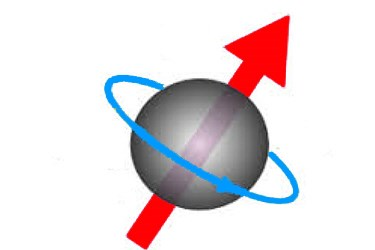
\includegraphics[width=55mm, height=40mm]{spin}
\captionof{figure}{Vjerojatnosti pronalaženja qbita u određenom stanju opisano je njegovim kvantnim stanjem (spinom).}
\end{center}

\paragraph{}
Sustavi s kvantnim bitovima mogu biti definirani za proizvoljan brojevni sustav, no kako su današnja računala bazirana na binarnom brojevnom sustavu zanima nas definicija qbita s 2 stanja.

\subsection{Blochova shema}
\paragraph{}
Stanje qbita prikazujemo Blochovom shemom. Jedno kvantno stanje prikazujemo kao vektor iz središta sfere na njezinu površinu. Stanja u kojima pronalazimo česticu prikazujemo polovima sfere koje definiramo sjecištima sfere i z-osi.

\begin{center}
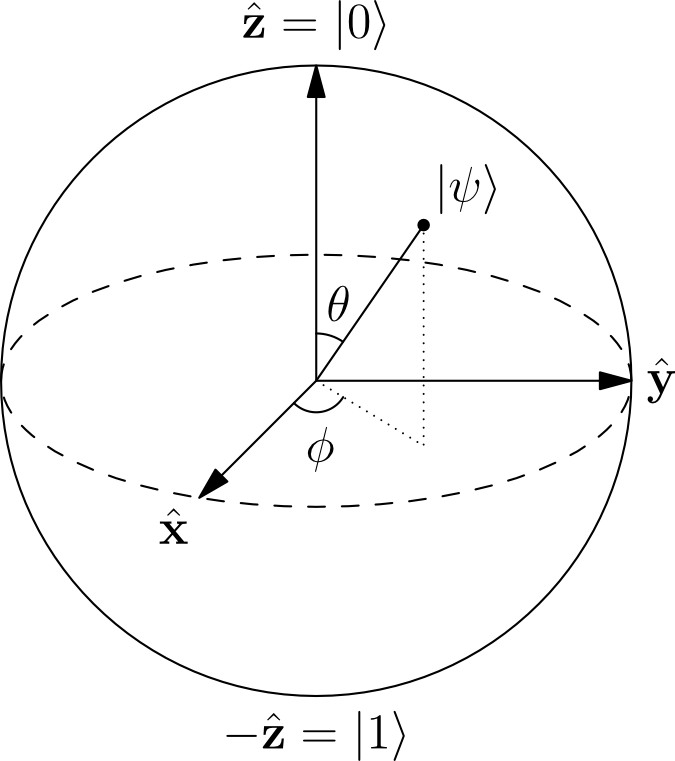
\includegraphics[width=60mm, height=65mm]{bloch}
\captionof{figure}{Blochova sfera}
\end{center}

\paragraph{}
Na slici vidimo jedno kvantno stanje opisano vektorom. Matematički ga možemo opisati formulom:

\subparagraph{
$ \ket{\psi} = \alpha\ket{0} + \beta\ket{1} $
}

%%%%%%%%%%%%%%%%%%%%%%% Kompleksna def. alfe i bete

\paragraph{}
$\alpha$ i $\beta$ predstavljaju gustoće vjerojatnosti pronalaženja qbita u stanju $\ket{0}$ i $\ket{1}$ respektivno. Iz gustoća vjerojatnosti računamo vjerojatnosti pronalaženja qbita u jednom od stanja:

\begin{equation} \label{eql}
\begin{split}
\Pr{\ket{0}} = \alpha^{2} = \cos^{2}{\frac{\theta}{2}} \\ 
\Pr{\ket{1}} = \alpha^{2} = \sin^{2}{\frac{\theta}{2}}
\end{split}
\end{equation}

\subsection{Aproksimacija}
Pojednostavljenje, matematika, matrice...

\subsection{Korištena aproksimacija}
Definicija krajnje aproksimacije...
\section{Kvantni registar}
Kvantni registar, poput klasičnog registra, sadrži niz qbit-ova.

\newpage

\chapter{Genetski algoritam inspiriran kvantnom mehanikom}
\section{Klasični genetski algoritam (CGA)}
\subsection{Djelovi}
Klasični genetski algoritam zahtjeva nekoliko osnovnih dijelova:
\begin{itemize}
\item Genotip 
\item Operator križanja 
\item Operator mutacije
\item Evaluator 
\end{itemize}

\subsection{Pseudokod}
U ovom primjeru gledamo pseudokod turnirskog algoritma s konstantnom veličinom populacije (SteadyStateTournament).
%\begin{algorithmic}
%\Call{InitializePopulation}{0}
%\If {$i\geq maxval$}
%    \State $i\gets 0$
%\Else
%    \If {$i+k\leq maxval$}
%        \State $i\gets i+k$
%    \EndIf
%\EndIf
%\end{algorithmic}

\section{Genetski algoritam inspiriran kvantnom mehanikom}
\subsection{Djelovi}
Genetski algoritam inspiriran kvantnom mehanikom uz svoje specifične operatore sadrži i dijelove slične onima iz CGA:
\begin{itemize}
\item Kvantni genotip (kvantni registar)
\item Kvantni operator križanja 
\item Kvantni operator mutacije
\item Operator kvantnih rotacijskih vrata
\item Evaluator
\end{itemize}
\subsection{Pseudokod}
\subsection{Rad algoritma}
\subsection{Implementacijski detalji}


\newpage

\chapter{Primjena}
\section{Traženje globalnog minimuma funkcije (FunctionMin)}
\subsection{Opis problema}
Zadane su netricijalne funkcije u 3 dimenzije kojima je potrebno pronaći točku minimuma.
Zadane funkcije:
\begin{itemize}
\item Kvadratna
\item Schaffer-ova F6 funkcija
\item Griewangk
\item Ackley
\item Rastrigin
\item Rosenbrock
\item Schaffer-ova F6 funkcija
\end{itemize}

\subsection{Rezultat}

\section{Knapsack problem}
\subsection{Opis problema}
Zadana je nosivost torbe (knapsack) i popis stvari i njima pripadnih težina.
Potrebno je pronaći najbolju kombinaciju stvari uz uvijet da je zadovoljena nosivost torbe.

\subsection{Rezultat}

\section{Regresija neuronske mreže}
\subsection{Opis problema}
Za zadane ulaz/izlaz podatke potrebno je pronaći težine veza neuronske mreže (učenje neuronske mreže).

\subsection{Rezultat}

\section{COCO}
\subsection{Opis problema}
Usporedba s ostalim optimizacijskim algoritmima

\subsection{Rezultat}

\newpage

\chapter{Moguća nadogradnja}
\section{Paralelizacija}
Stvaranjem više nezavisnih populacija jedinki te povremenom razmjenom najboljih jedinki između populacija poboljšava se rad algoritma.

\section{Podržavanje više-genotipskih jedinki}
Trenutno je ostvarena podrška jedinki s jednim genotipom. Podršku više genotipa moguće je ostvariti izmjenom 'prilagodnika' unutar algoritma te prikladnim zastavicama za odabir genotipa koji će poprimati vrijednosti kvantnog registra.

\newpage

\chapter{Zaključak}
Kolko je isplativ GAIQM?

\bibliography{literatura}
\bibliographystyle{fer}

\begin{sazetak}
Cilj rada je objasniti koncept pohrane i manipulacije podacima na kvantnim računalima, mogućnost primjene na genetske algoritme na klasičnim računalima te proširenje ECF-a dotičnim algoritmom. Algoritam je primjenjen na 3 različita problema (traženje minimuma, knapsack, regresija neuronske mreže). Rezultati ukazuju na ...

\kljucnerijeci{genetski algoritam, kvantna mehanika, qbit, knapsack, neuronska mreža}
\end{sazetak}

\engtitle{Genetic algorithm inspired by quantum mechanics}
\begin{abstract}
ENGLISH

\keywords{genetic algorithm, quantum mechanics, qbit, knapsack, neural network}
\end{abstract}

\end{document}